\begin{document}
%\begin{CJK*}{GBK}{song}
\newcommand{\vect}[1]{\boldsymbol{#1}}

\def\lecturename{System Identification}

\title{\insertlecture}

\author{Xing Chao}

\institute
{
School of Astronautics, Northwestern Polytechnical University
}

%\mode<presentation>{\subject{嵌入式系统}}

%  start a lecture  --------------------------
\lecture[LTI]{Classical identification for linear time invariant systems}{}
\subtitle{}
\date{}


%\setbeamertemplate{background}{\pgfimage[width=\paperwidth,height=\paperheight]{image/flower}}
%\setbeamercovered{transparent}
%\mode<presentation>{\beamerdefaultoverlayspecification{<+->}}

\begin{frame}
  \maketitle
\end{frame}


\section{Basic concepts in classic identification}

%\begin{frame}{什么是经典辨识}
%由经典控制理论而来。经典控制中由三种典型输入信号可得三个典型输出,即
%\begin{itemize}
%\item  正弦输入—频率响应
%\item  阶跃输入—阶跃响应
%\item  脉冲输入—脉冲响应
%\end{itemize}
%% 在自动控制原理中,讲述了如何由它们来求解出系统的传递函数。
%\end{frame}

\begin{frame}{classical identification method definition}
A method for obtaining a mathematical model of a system from three classical input signals.
\begin{itemize}
\item sinusoidal input --- frequency response % - seeking transfer function;
\item step input --- step response % - seeking transfer function;
\item impulse input --- impulse response % - seeking transfer function;
\end{itemize}
The focus of this course is on the method of obtaining the mathematical model of the system by using the impulse input signal.
\end{frame}

\begin{frame}{Classic identification of content, purpose and method}
\begin{itemize}
\item Classic identification content and purpose:
\begin{itemize}
\item How to get the impulse response of the system?
\item How to determine the transfer function and impulse transfer function of the system from the impulse response of the system?
\end{itemize}
\item Solution:
\begin{itemize}
\item To get the impulse response of the system, use the correlation method;
\item To find the parameter model of the system from the impulse response, use pure analytical method.
\end{itemize}
\end{itemize}
\end{frame}


\begin{frame}{Correlation method to obtain the impulse response of the system: system model}
% \begin{tikzpicture}[scale=.8,auto=left]
% \node (g) [shape=rectangle,draw] {linear system ($g(\tau)$)};
% \node (s) [left of =g] {};
% \node (e) [right of =g] {};
% \tikzstyle{g}=[fill=red!20]
% \draw [->] (s) -- (g) node[midway] {$x(t)$};
% \draw [->] (g) -- (e) node[midway] {$y(t)$};
% \end{tikzpicture}

Refer to the SISO system impulse response function as $g(\tau)$. According to the convolution theorem of linear systems:
$$
y(t)=\int_{-\infty}^{\infty} g(\sigma)x(t-\sigma)d\sigma
$$
Let $x(t)$ be a stationary stochastic process with a mean of $0$, then $y(t)$ is also a stationary stochastic process with a mean of $0$. At any time, $t_2$, when $t=t_2$, the above formula is
$$
y(t_2)=\int_{-\infty}^{\infty} g(\sigma)x(t_2-\sigma)d\sigma
$$
Multiply the above formula with the input $x(t_1)$ at another time to get:
$$
x(t_1)y(t_2)=\int_{-\infty}^{\infty} g(\sigma)x(t_1)x(t_2-\sigma)d\sigma
$$
\end{frame}

\begin{frame}{Correlation method to obtain the impulse response of the system: Wiener-Hoff equation}
Take mathematics expectations on both sides and get:
$$
E[x(t_1)y(t_2)]=\int_{-\infty}^{\infty} g(\sigma)E[x(t_1)x(t_2-\sigma)]d\sigma
$$
The Wiener-Hoff equation can be obtained:
$$
R_{xy}(\tau)=\int_{-\infty}^{\infty} g(\sigma)R_x(\tau)]d\sigma
$$
Where: $\tau=t_2-t_1$
If $R_{xy}$ and $R_x$ are known in the equation, then the above equation can be solved to get $g(\tau)$
\end{frame}

\begin{frame}{Correlation method to obtain the impulse response of the system: Wiener-Hoff equation solving}
% However, in general, the above equation is extremely difficult to solve. Only in some special cases can the Wiener Hof equation be solved. Special case:
When $x(t)$ is a white noise signal, there is $R_x(\tau)=K\delta(\tau)$, and
$R_x(\tau-\sigma) = K\delta(\tau-\sigma)$

After substituting the Wiener Hof equation, it is available
\begin{eqnarray*}
R_{xy}(\tau) &=& \int_{-\infty}^{\infty}g(\sigma)K\delta(\tau-\sigma)d\sigma \\
&=& Kg(\tau) \\
g(\tau)&=& \frac{R_{xy}(\tau)}{K}
\end{eqnarray*}
For the solution of $g(\tau)$, just calculate $R_{xy}$. If the observation time $T_m$ is sufficiently large, then
\begin{eqnarray*}
R_{xy}(\tau) &=& \frac{1}{T_m}\int_0^{T_m}x(t)y(t+\tau)dt \\
R_{xy}(k) &=& \frac{1}{N}\sum_{i=0}^{N-1}x_i y_{i+k}
\end{eqnarray*}
Where $x_i, y_{i+k}$ is the sequence of data recorded.
\end{frame}

\section{commonly used input signals in identification}
\begin{frame}{white noise process}
If the mean of the random process $w(t)$ is 0, the autocorrelation function is:
$$
R_w(t)=\sigma^2\delta(t)
$$
The process is called a white noise process.
among them:
$$
\delta(t)=\begin{cases}
\infty & t=0 \\ 0 & t\neq 0
\end{cases}
$$
\end{frame}

\begin{frame}{Problems in the engineering practice}
\begin{itemize}
\item To use impulse input to get impulse response, is not possible in engineering
\item white noise is artificially unproducible in engineering;
\end{itemize}
Therefore, the system's impulse response sequence must be identified by an input signal that can be repeatedly generated in the engineering practice.
\begin{itemize}
\item pseudo-random noise;
\item discrete two-bit white noise sequence;
\item pseudo-random discrete two-bit sequence; (M-sequence)
\item two-level M sequence;
\end{itemize}
\end{frame}

\begin{frame}{Pseudo-random noise identification impulse response}
Pseudorandom noise is truncated by white noise and is a periodic signal.
\begin{eqnarray*}
R_x(\tau) &=& R_x(\tau+T) \\
&=& \delta(nT+\tau)
\end{eqnarray*}
Where $n=0,\pm 1,\pm 2,\cdots$
\end{frame}

\begin{frame}{Pseudo-random noise identification impulse response: Calculate $R_{xy}$}
Pseudo-random noise signals as input signals , then:
\begin{eqnarray*}
R_{xy} &=& \int_{-\infty}^{\infty} g(\sigma)R_x(\tau-\sigma)d\sigma \\
&=& \int_{0}^{T}g(\sigma)R_x(\tau-\sigma)d\sigma+\int_{T}^{2T}g(\sigma)R_x(\tau-\sigma)d\sigma +\cdots \\
&=& \int_0^T g(\sigma)K\delta(\tau-\sigma)d\sigma+\int_T^{2T}g(\sigma)K\delta(T+\tau-\sigma)d\sigma \\
&& +\cdots \\
&=& Kg(\tau)+Kg(\tau+T)+Kg(\tau+2T)+\cdots
\end{eqnarray*}
\end{frame}

\begin{frame}{Pseudorandom noise identification impulse response: Calculate $g(\tau)$}
Select the appropriate truncation period so that $g(\tau)$ has decayed to zero at $\tau<T$. then:
\begin{eqnarray*}
R_{xy}(\tau)&=& K g(\tau)+0 \\
&=& Kg(\tau) \\
g(\tau)&=& R_{xy}(\tau)/K
\end{eqnarray*}
The same identification result as white input is obtained.
\end{frame}

\begin{frame}{Calculate $R_x(\tau),R_{xy}(\tau)$}
\begin{eqnarray*}
R_x(\tau) &=& \lim_{n \rightarrow \infty}\frac{1}{nT}\int_0^{nT}x(t)x(t+\tau)dt \\
&=&\lim_{n\rightarrow \infty}\frac{n}{nT}\int_0^{T}x(t)x(t+\tau)dt \\
&=&\frac{1}{T}\int_0^{T}x(t)x(t+\tau)dt \\
R_{xy}(\tau) &=& \int_{-\infty}^{\infty}g(\sigma)R_x(\tau-\sigma)d\sigma \\
&=& \int_{-\infty}^{\infty}g(\sigma)\left[\frac{1}{T}\int_0^Tx(t)x(t+\tau-\sigma)dt\right]d\sigma \\
&=& \frac{1}{T}\int_0^T x(t)\left[\int_{-\infty}^{\infty}g(\sigma)x(t+\tau-\sigma)d\sigma\right]dt \\
&=& \frac{1}{T}\int_0^T x(t)y(t+\tau)dt
\end{eqnarray*}
 $R_{xy}(\tau)$ only needs one cycle calculation.
\end{frame}

\begin{frame}{discrete white noise}
A random sequence of consecutive white noise samples at equal intervals. Has the same statistical properties of continuous white noise, ie
$$
E(x_i x_j) =\begin{cases} \sigma^2 & i=j \\
0 & i\neq j\end{cases}
$$
Where $i,j=1,2,3,\cdots$
\end{frame}

\begin{frame}{discrete two-bit white noise}
Discrete random variables take only two values. The elements in the sequence are generally taken as 1 and -1
%, also the true white noise, using it as the input signal, the result of identifying $g(\tau)$ is exactly the same as the continuous white noise.

Example: a discrete two-bit noise

          1111-1-1-11-1-111-11-1···

Main properties:
\begin{itemize}
\item -1 and 1 appear equal times;
\item The total number of  total runs (the segments in which the states "1" and "-1" appear consecutively are called runs) are (N+1)/2, and the runs of -1 and 1 are equal, up to one difference. (N is the length of the sequence)
\item its autocorrelation function is
$$
R_{xx}(\tau) =\begin{cases} 1 & \tau=0 \\
0 & \tau \neq 0 \end{cases}
$$
\end{itemize}
\end{frame}

\begin{frame}{Features of the M sequence}
In engineering practice, the M sequence is often used instead of the white noise input signal to identify the impulse response sequence of the system. Features of the M sequence:
\begin{itemize}
\item pseudo-random two-position sequence;
\item The digital features of the  M sequence are similar to white noise;
\item deterministic sequence;
\item can be easily regenerated in engineering practice.
\end{itemize}
\end{frame}

\begin{frame}{M sequence generation method and its properties}
M sequence: A pseudo-random sequence constructed by truncating a discrete two-bit noise sequence.
Notable features:
\begin{itemize}
\item M sequence is a deterministic sequence that can be repeated;
\item M sequence has similar properties to discrete two-bit white noise.
\end{itemize}
Producing method: The M sequence is generated by engineering using the shift register method.
\begin{eqnarray*}
X_0(k+1)&=&a_0 x_0(k) \oplus a_1 x_1(k)\oplus \cdots \oplus a_n x_n(k) \\
X_1(k+1)&=& x_0(k) \\
&& \cdots \\
X_n(k+1)&=& x_{n-1}(k)
\end{eqnarray*}
Pseudo-random sequence generating conditions : the initial state of each register is not all zero.
\end{frame}


\begin{frame}{M sequence generation method and its properties}
example:
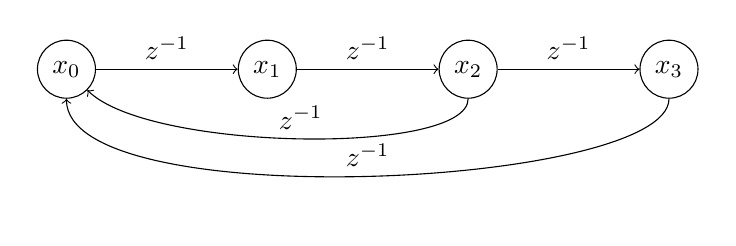
\begin{tikzpicture}
\matrix[ampersand replacement=\&,row sep=0.5cm, column sep=1.8cm]{
\node[draw,circle] (x0) {$x_0$}; \& \node [draw,circle](x1) {$x_1$}; \& \node [draw,circle](x2) {$x_2$};  \& \node[draw,circle](x3) {$x_3$}; \\ };
\draw[->] (x0) --node[above, midway]{$z^{-1}$}(x1);
\draw[->] (x1) --node[above, midway]{$z^{-1}$}(x2);
\draw[->] (x2) --node[above, midway]{$z^{-1}$}(x3);
\draw[->] (x2).. controls +(-90:1.1cm) and +(-45:1.1cm) ..  node[above, midway]{$z^{-1}$} (x0.south east);
\draw[->] (x3).. controls +(-90:1.5cm) and +(-90:1.5cm) ..  node[above, midway]{$z^{-1}$} (x0.south);
\end{tikzpicture}
\begin{eqnarray*}
x_0(k+1)&=& x_2(k)\oplus x_3(k) \\
x_1(k+1)&=& x_0(k) \\
x_2(k+1)&=& x_1(k) \\
x_3(k+1)&=& x_2(k)
\end{eqnarray*}
\end{frame}

\begin{frame}[containsverbatim]{M sequence methods and their properties}
When the initial state is all 1, the status of each register is
\begin{verbatim}
X0: 100010011010111
X1: 110001001101011
X2: 111000100110101
X3: 111100010011010
\end{verbatim}
%\begin{itemize}
%\item 1111 (initial state)→0111→0011→0001→1000 →
%\item 0100 → 0010 → 1001 → 1100 →
%\item 0110 →1011→0101→1010→1101→1110→1111
%\end{itemize}
The output sequence is: 111100010011010 (length N=15)
\end{frame}

\begin{frame}{M sequence generation method and its properties}
If the number of registers is n, then there is
\begin{itemize}
\item period length $N=2^n-1$;
\item total run = $2^{n-1}$ ;
\item The number of occurrences of  "0" is (N-1)/2, and the number of occurrences of "1" is (N+1)/2. The difference is 1 time.
\end{itemize}
\end{frame}

\begin{frame}{two-level M sequence and its properties}
\begin{itemize}
\item turns the M sequence into a level signal,
\begin{itemize}
\item "0" is taken as a, and "1" is taken as -a.
The \item shift pulse period is $\Delta$, and the period of the two-level M sequence is $N\Delta$.
\end{itemize}
\item numeric features:
In a period of $N\Delta$, its mean $m_x$ is \\
\begin{eqnarray*}
M_x &=& \frac{1}{N\Delta}\left(\frac{N-1}{2}a\Delta-\frac{N+1}{2}a\Delta\right)=-\frac{a}{N} \\
\lim_{N\rightarrow \infty}m_x &=& 0
\end{eqnarray*}
\end{itemize}
\end{frame}

\begin{frame}{autocorrelation function $R_x(\tau)$}
$$
R_x{\tau}=\begin{cases}
\displaystyle \frac{-a^2}{N} & \scriptstyle (kN+1)\Delta<\tau<((k+1)N-1)\Delta  \\
\displaystyle a^2\left[ 1-\frac{(N+1)|\tau|}{N\Delta}\right] &\scriptstyle (kN-1)\Delta<\tau<(kN+1)\Delta
\end{cases}
$$
\end{frame}

\begin{frame}{Triangular impulse component and DC component}
$$
R_x(\tau)=R^1_x(\tau)+R^2_x(\tau)
$$
where:
\begin{description}
\item[$R_x^2(\tau)=\frac{-a^2}{N}$]is DC component
\item[$R_x^1(\tau)=R_x(\tau)-R^2_x(\tau)$]is triangular pulse component
\end{description}
\end{frame}

\begin{frame}
When $\Delta$ is small, $R_x^1(\tau)$ can be considered as a impulse function, then there is
\begin{eqnarray*}
R_x^1(\tau) &=& \frac{N+1}{N}a^2\Delta\delta(\tau) \\
R_x(\tau) &=& \frac{N+1}{N}a^2\Delta\delta(\tau)-\frac{a^2}{N}
\end{eqnarray*}
Therefore, the M sequence has a digital characteristic of a white noise sequence.
\end{frame}


\section{M sequence  identify the impulse response of the system}

\begin{frame}{ two-level M-sequence recognize system impulse response sequence $g(\tau)$ : graphical method}
The two-level M-sequence recognizes $g(\tau)$ in two ways: the graphical method and the formula method. First introduce the graphical method:
\begin{eqnarray*}
R_{xy}(\tau) &=&  \int_{-\infty}^{\infty}g(\sigma)R_x(\tau-\sigma)d\sigma  \\
&=& \int_{0^+}^{N\Delta^-}g(\sigma)R_x(\tau-\sigma)d\sigma \\
&=& \int_{0^+}^{N\Delta^-}\left[\frac{N+1}{N}a^2\Delta\delta(\tau-\sigma)-\frac{a^2}{N}\right]g(\sigma)d\sigma \\
&=& \frac{N+1}{N}a^2\Delta g(\tau)-\int_{0^+}^{N\Delta^-}g(\sigma)d\sigma \\
&=& \frac{N+1}{N}a^2\Delta g(\tau)-A 
\end{eqnarray*}
where:
$
A=\int_{0^+}^{N\Delta^-}g(\sigma)d\sigma 
$
\end{frame}

\begin{frame}
$R_{xy}(\tau)$ can be calculated from the input and output data sequence:
$$
R_{xy}(\tau)=\frac{1}{N}\sum_{i=1}^{N-1}x(i)y(i+\tau)
$$
Simply pan the $R_{xy}(\tau)$ curve up by A to get $g(\tau)$.
%$$(\tau)\rightarrow 0$ when $\tau\rightarrow \infty$
\end{frame}

\begin{frame}{Analytical method to get $g(\tau)$}
\begin{eqnarray*}
R_{xy}(\tau) &=& \frac{N+1}{N}a^2\Delta g(\tau)-\frac{a^2}{N}\int_0^{N\Delta}g(\sigma)d\sigma \\
\int_0^{N\Delta}R_{xy}(\tau)d\tau &=& \frac{N+1}{N}a^2\Delta \int_0^{N\Delta}g(\tau)d\tau \\
&& -\frac{a^2}{N}N\Delta\int_0^{N\Delta}g(\sigma)d\sigma \\
&=&\frac{\Delta a^2}{N}\int_0^{N\Delta}g(\tau)d\tau  \\
R_{xy}(\tau) &=& \frac{N+1}{N}a^2\Delta g(\tau)-\frac{1}{\Delta}\int_0^{N\Delta}R_{xy}(\sigma)d\sigma \\
g(\tau)&=&\frac{N}{(N+1)\Delta a^2}\left[R_{xy}(\tau)+\frac{1}{\Delta}\int_0^{N\Delta}R_{xy}(\sigma)d\sigma\right]
\end{eqnarray*}
\end{frame}

\begin{frame}{Analytical method to get $g(\tau)$}
\begin{eqnarray*}
g(\tau)&=&\frac{N}{(N+1)\Delta a^2}R_{xy}(\tau) +g_0\\
g_0 &=& \frac{N}{(N+1)\Delta^2 a^2}\int_0^{N\Delta}R_{xy}(\tau)d\tau \\
\int_0^{N\Delta}R_{xy}(\tau)d\tau &\approx & \Delta\sum_{i=0}^{N-1}R_{xy}(i) \\
R_{xy}(\tau) &=& \frac{1}{N}\sum_{i=0}^{N-1}x(i)y(i+\tau)
\end{eqnarray*}
\end{frame}

\begin{frame}{Matrix representation for $g(\tau)$}
Discrete Wiener-Hoff equation:
\begin{eqnarray*}
R_{xy}(i\Delta) &=& \sum_{k=0}^{N-1}\Delta g(k\Delta)R(i\Delta-k\Delta) \\
R_{xy} &=& R g\Delta  \\
g&=& \frac{R^{-1} R_{xy}}{ \Delta }
\end{eqnarray*}
where:
\begin{eqnarray*}
g &=& [g(0),g(1),\cdots,g(N-1)]^T \\
R_{xy} &=& [R_{xy}(0),R_{xy}(1),\cdots,R_{xy}(N-1)]^T \\
R &=&
\begin{bmatrix}
R_x(0) & R_x(-1)  & \cdots & R_x(-N+1)  \\
R_x(1) & R_x(0)   & \cdots & R_x(-N+2)  \\
\vdots & \vdots   &        & \vdots     \\
R_x(N-1) & R_x(N-2)   & \cdots & R_x(0)  
\end{bmatrix}
\end{eqnarray*}
\end{frame}

\begin{frame}{Matrix representation for $g(\tau)$ :calculate $R^{-1}$ }
\begin{eqnarray*}
R_x(k) &=&
\begin{cases}
a^2 & k=0  \\
-\frac{a^2}{N}  & 1\leq k \leq N-1
\end{cases} \\
R &=& a^2
\begin{bmatrix}
1 & -\frac{1}{N} & \cdots & -\frac{1}{N}  \\
-\frac{1}{N} & 1 & \cdots & -\frac{1}{N}  \\
\vdots & \ddots  & \ddots & \vdots \\
-\frac{1}{N} & -\frac{1}{N} & \cdots & 1 
\end{bmatrix} \\
R^{-1} &=& \frac{N}{a^2(N+1)}
\begin{bmatrix}
2 & 1 & \cdots & 1 \\
1 & 2 & \cdots & 1 \\
\vdots & \vdots & \vdots & \vdots \\
1 & 1 & \cdots  & 2
\end{bmatrix}
\end{eqnarray*}
\end{frame}

\begin{frame}{Matrix representation for $g(\tau)$:calculate $R_{xy}$}
\begin{eqnarray*}
R_{xy} &=& [R_{xy}(0),R_{xy}(1),\cdots,R_{xy}(N-1)]^T \\
&=&  \frac{1}{rN}XY \\
X&=&
\begin{bmatrix}
x(0) & x(1) & \cdots & x(rN-1) \\
x(-1) & x(0) & \cdots & x(rN-2) \\
\vdots & \vdots &  & \vdots \\
x(-N+1) & x(-N+2) & \cdots & x(rN-N) 
\end{bmatrix}\\
Y &=& \begin{bmatrix} y(0) & y(1) &\cdots & y(rN-1) \end{bmatrix}^T
\end{eqnarray*}
\end{frame}


\begin{frame}{ Recursive algorithm for $g(\tau)$ (online identification)}
Recursive algorithm: Suppose we get the identification result $g_{m-1}$ for the $(m-1)$ observations, and now we have a new set of observations $(x_m,y_m)$. Now let's discuss how to get the new $g(\tau)$ estimate $g_m$ for $g_{m-1}$ and $(x_m,y_m)$ data.

The formula for the general recursive algorithm is as follows:
$$
G_m = K g_{m-1} + \tilde{g}_m
$$
Among them, $\tilde{g}_m$ is the information added from the newly obtained data.
\end{frame}

\begin{frame}{Recursive formula for $R_{xy}$}
\begin{eqnarray*}
R_{xy}(i,m) &=& \frac{1}{m+1}\sum_{k=0}^m y(k)x(k-i) \\
&=& \frac{1}{m+1}\left[\sum_{k=0}^{m-1} y(k)x(k-i)+y(m)x(m-i)\right] \\
&=& \frac{1}{m+1}\left[mR_{xy}(i,m-1)+y(m)x(m-i)\right] \\
R_{xy}(m)&=& \frac{1}{m+1}\left[mR_{xy}(m-1)+y(m)X(m)\right] %\\
\end{eqnarray*}
where:
\begin{eqnarray*}
R_{xy}(m) &=& [R_{xy}(0), R_{xy}(1), \cdots, R_{xy}(N-1)]^T \\
X(m) &=& [x(m),x(m-1),\cdots,x(m-N+1)]^T
\end{eqnarray*}
\end{frame}

\begin{frame}{Recursive formula for $g(\tau)$}
\begin{eqnarray*}
g_m &=& \frac{R^{-1}R_{xy}(m)}{\Delta} \\
&=& \frac{R^{-1}}{\Delta}\frac{1}{m+1}\left[mR_{xy}(m-1)+y(m)X(m)\right] \\
&=& \frac{mR^{-1}R_{xy}(m-1)}{(m+1)\Delta}+\frac{R^{-1}}{(m+1)\Delta}y(m)X(m) \\
&=& \frac{m}{m+1}g_{m-1}+\frac{R^{-1}}{(m+1)\Delta}y(m)X(m) %\\
\end{eqnarray*}
\end{frame}

%    \begin{frame}{$g(\tau)$的矩阵表示}
%    在系统输入(r+1)个周期二电平M序列时,有
%    \begin{eqnarray*}
%    g &=& \frac{1}{a^2 r(N+1)\Delta}
%    \begin{bmatrix}
%    2 & 1 & \cdots & 1 \\
%    1 & 2 & \cdots & 1 \\
%    \vdots & \vdots & \vdots & \vdots \\
%    1 & 1 & \cdots  & 2
%    \end{bmatrix}
%    XY
%    \end{eqnarray*}
%    其中:
%    \begin{eqnarray*}
%    g &=&  \begin{bmatrix} g(0) & g(1) & \cdots & g(N-1) \end{bmatrix}^T  \\
%    X &=&  \begin{bmatrix}
%    x(0) & x(1) & \cdots & x(rN-1) \\
%    x(-1) & x(0) & \cdots & x(rN-2) \\
%    \vdots & \vdots & \vdots & \vdots \\
%    x(-N+1) & x(-N+2) & \cdots & x(rN-N) 
%    \end{bmatrix} \\
%    Y &=& \begin{bmatrix} y(0) & y(1) & \cdots & y(rN-1) \end{bmatrix}^T
%    \end{eqnarray*}
%    \end{frame}
%    
%    
%    \begin{frame}{$g(\tau)$的递推算法(在线辨识)}
%    递推算法:假设我们得到了$(m-1)$组观测数据时的辨识结果$g_{m-1}$,现在又得到了一组新的观测值$(x_m,y_m)$。现在讨论,就$g_{m-1}$与$(x_m,y_m)$数据来如何得到新的$g(\tau)$估计值$g_m$问题。
%    
%    一般递推算法的计算公式形式如下:
%    $$
%    g_m = K g_{m-1} + \tilde{g}_m
%    $$
%    其中,$\tilde{g}_m$为利用新观测值对g的预测值。
%    \end{frame}
%    
%    \begin{frame}{$R_{xy}$递推公式}
%    \begin{eqnarray*}
%    R_{xy}(i,m) &=& \frac{1}{m+1}\sum_{k=0}^m y(k)x(k-i) \\
%    &=& \frac{1}{m+1}\left[\sum_{k=0}^{m-1} y(k)x(k-i)+y(m)x(m-i)\right] \\
%    &=& \frac{1}{m+1}\left[mR_{xy}(i,m-1)+y(m)x(m-i)\right] \\
%    %&=& R_{xy}(i,m-1)+ \frac{1}{m+1}\left[-R_{xy}(i,m-1)+y(m)x(m-i)\right] 
%    R_{xy}(m)&=& \frac{1}{m+1}\left[mR_{xy}(m-1)+y(m)X(m)\right] %\\
%    \end{eqnarray*}
%    其中:
%    $$
%    X_m=[x(m),x(m-1),\cdots,x(m-N+1)]^T
%    $$
%    \end{frame}
%    
%    \begin{frame}{$g(\tau)$递推公式}
%    \begin{eqnarray*}
%    g_m &=& \frac{1}{rN\Delta}R^{-1}R_{xy}(m) \\
%    &=& \frac{R^{-1}}{rN\Delta}\frac{1}{m+1}\left[mR_{xy}(m-1)+y(m)X(m)\right] \\
%    &=& \frac{1}{m+1}\left[m\frac{R^{-1}}{rN\Delta}R_{xy}(m-1)+\frac{R^{-1}}{rN\Delta}y(m)X(m)\right] \\
%    &=& \frac{m}{m+1}g_{m-1}+\frac{R^{-1}}{(m+1)rN\Delta}y(m)X(m) %\\
%    % &=&  \frac{1}{rN\Delta} R^{-1} \{R_{xy}(m-1)\\
%    % && +\frac{1}{m+1}\left[-R_{xy}(m-1)+y(m)X_m\right]\} \\
%    % &=& g_{m-1}+  \frac{1}{m+1}\left[\frac{1}{rN\Delta}R^{-1}X_m y(m)-g_{m-1}\right] 
%    \end{eqnarray*}
%    \end{frame}

\section{from impulse response sequence to get  system G(s) and G(z)}
\begin{frame}{Impulse response sequence for G(z)}
G(z) is called the pulse transfer function of the system and is a discrete mathematical model of the system.
\begin{eqnarray*}
G(z)&=&\frac{C(z)}{R(z)}  \\
&=&\frac{b_0+b_1 z^{-1}+\cdots+b_n z^{-n}}{1+a_1 z^{-1}+\cdots+a_n z^{-n}}
\end{eqnarray*}
get:
\begin{eqnarray*}
c_t+a_1 c_{t-1}+\cdots+ a_n c_{t-n} =  b_0 r_t+ \cdots + b_n r_{t-n}  \\
g(t)+a_1 g(t-1)+\cdots+ a_n g(t-n) =  b_0 \delta(t)+ \cdots + b_n \delta(t-n)
\end{eqnarray*}
\end{frame}

\begin{frame}
$$
\begin{bmatrix}
b_0 \\
b_1 \\
\vdots \\
b_0 
\end{bmatrix}
=
\begin{bmatrix}
1 & 0 & \cdots & 0 \\
a_1 & 1 & \cdots & 0 \\
\vdots & \ddots & \ddots & \vdots \\
a_n & a_{n-1} & \cdots & 1
\end{bmatrix}
\begin{bmatrix}
g(0) \\
g(1) \\
\vdots \\
g(n)
\end{bmatrix}
$$

$$
\begin{bmatrix}
g(1) & g(2) & \cdots & g(n)  \\
g(2) & g(3) & \cdots & g(n+1) \\
\vdots & \vdots &  & \vdots \\
g(n) & g(n+1) & \cdots & g(2n-1)
\end{bmatrix}
\begin{bmatrix}
a_n \\
a_{n-1} \\
\vdots \\
a_1
\end{bmatrix}
=
\begin{bmatrix}
-g(n+1) \\
-g(n+2) \\
\vdots  \\
-g(2n)
\end{bmatrix}
$$
\end{frame}

\begin{frame}{use impulse response sequence to get G(s)}
G(s) is called the transfer function of the system and is a continuous mathematical model of the system.
$$
G(s)=\frac{C(s)}{R(s)}=\frac{M(s)}{N(s)}
$$

If the system has n closed-loop poles $s_1, s_2, \cdots, s_n$.
Then the above formula can be divided into:
$$
G(s)=\frac{c_1}{s-s_1}+\frac{c_2}{s-s_2}+\cdots+\frac{c_n}{s-s_n}
$$
Task: $\{g(i)\}$ and $n$ are known, find $G(s)$ in the coefficients $c_i$ and $s_i$.
\end{frame}

\begin{frame}{calculate $a_i$}
System impulse transfer function is 
$$
G(z)=\frac{b_0+b_1 z+ \cdots b_n z^n}{1+a_1 z + \cdots + a_n z^n}
$$
let $r(t)=\delta(t)$, then $c(t)=g(t)$。Substituting the above formula, write the difference equation as
$$
g(k)+a_1g(k+1)+\cdots+a_ng(k+n) = 0
$$
get:
\begin{eqnarray*}
a_1g(k+1)+\cdots+a_ng(k+n) &=& -g(k) \\
\cdots &&  \\
a_1g(k+n)+\cdots+a_ng(k+2n-1) &=& -g(k+n-1)
\end{eqnarray*}
solving above linear equation of $n$ unknowns , get $a_i$.
\end{frame}

\begin{frame}{calculate $s_i$}
The inverse Laplace transform from $G(s)$ gives:
$$
g(t)=c_1 e^{s_1 t} + c_2 e^{s_2 t} + ... + c_n e^{s_n t}
$$
so:
\begin{eqnarray*}
g(t) &=& c_1 e^{s_1 (t)} + c_2 e^{s_2 (t)} + ... + c_n e^{s_n (t)}  \\
g(t+\Delta) &=& c_1 e^{s_1 (t+\Delta)} + c_2 e^{s_2 (t+\Delta)} + ... + c_n e^{s_n (t+\Delta)}  \\
\cdots && \cdots \\
g(t+n\Delta) &=& c_1 e^{s_1 (t+n\Delta)} + c_2 e^{s_2 (t+n\Delta)} + ... + c_n e^{s_n (t+n\Delta)}  \\
0 &=& c_1 e ^{s_1 t}[1+a_1 e^{s_1 \Delta} + \cdots + a_n e^{s_1 n\Delta}]  \\
&& +c_2 e ^{s_2 t}[1+a_1 e^{s_2 \Delta} + \cdots + a_n e^{s_2 n\Delta}] +\cdots  \\
&& +c_n e ^{s_n t}[1+a_1 e^{s_n \Delta} + \cdots + a_n e^{s_n n\Delta}] 
\end{eqnarray*}
the linear equation of $n$ unkowns is required for  $e^{s_i\Delta}$:
$$
1+a_1 e^{s_i \Delta} +a_2 [e^{s_i\Delta}]^2+\cdots+a_n[e^{s_i\Delta}]^n=0
$$
where $i=1,2,\cdots,n$
\end{frame}

\begin{frame}{calculate $c_i$}
$$
g(t)=c_1 e^{s_1 t} + c_2 e^{s_2 t} + ... + c_n e^{s_n t}
$$
get :
\begin{eqnarray*}
g(0)&=& c_1 + c_2 + \cdots c_n \\
g(1)&=& c_1 e^{s_1 \Delta} + c_2 e^{s_2 \Delta}+\cdots+c_n e^{s_n \Delta} \\
&& \cdots \\
g(n-1)&=& c_1 e^{s_1 (n-1)\Delta} + c_2 e^{s_2 (n-1)\Delta}+\cdots+c_n e^{s_n (n-1)\Delta} \\
\end{eqnarray*}
\end{frame}

\begin{frame}{solution formula}
\begin{eqnarray*}
\begin{bmatrix}
g(k+1) & \cdots & g(k+n) \\
g(k+2) & \cdots & g(k+n+1) \\
\vdots & \vdots & \vdots \\
g(k+n) & \cdots & g(k+2n-1)
\end{bmatrix}
\begin{bmatrix}
a_1 \\ \vdots \\ a_n
\end{bmatrix}
&=&
\begin{bmatrix}
-g(k) \\ -g(k+1) \\  \vdots \\  -g(k+n-1)
\end{bmatrix} \\
1+a_1 x + \cdots a_n x^n &=& 0  \\
s_i&=&\frac{\ln x_i}{\Delta}  \\
\begin{bmatrix}
1 & 1 & \cdots & 1 \\
x_1 & x_2 & \cdots & x_n \\
\vdots & \vdots & \cdots & \vdots \\
x_1^{n-1} & x_2^{n-1} & \cdots & x_n^{n-1} \\
\end{bmatrix}
\begin{bmatrix}
c_1 \\ c_2 \\  \vdots \\ c_n
\end{bmatrix}
&=&
\begin{bmatrix}
g(0) \\ g(1) \\  \vdots \\  g(n-1)
\end{bmatrix}
\end{eqnarray*}

\end{frame}
% \section{思考}
% \begin{frame}{思考}
% \begin{itemize}
% \item 极大似然法辨识思想
% \end{itemize}
% \end{frame}


%\end{CJK*}
\end{document}
